\chapter{Lecture 19 - Numeric Integration with Newton-Cotes Formulas}
\label{ch:lec19n}
\section{Objectives}
The objectives of this lecture are to:
\begin{itemize}
\item Describe and illustrate the Midpoint and Trapezoidal ``rules'' for numeric integration
\item Demonstrate Simpson's Rule
\item Introduce and demonstrate \emph{numerical quadrature} for deriving integration formulas
\end{itemize}
\setcounter{lstannotation}{0}

\section{Newton-Cotes Integration Formulas}
Suppose you have a function, $f(x)$, that you want to integrate but, for some reason, you do not know how.  In addition to the more-or-less broad category of functions that you do not know how to integrate analytically, we can add the, perhaps, equally broad class of functions that simply cannot be integrate analytically at all by anyone.  One strategy for dealing with this situation is to:
\begin{enumerate}
\item Replace $f(x)$ with some other function $g(x)$ that you \emph{can} integrate.
\item If $g(x)$ is in some sense ``close'' to $f(x)$, you might hope that the integral of $g(x)$ would serve as a decent approximation to the integral of $f(x)$.
\end{enumerate}

This is the strategy followed for the Newton-Cotes integration formulas.  Each of the formulas in this class is distinguished from the others by the function $g(x)$ that the method used to approximate $f(x)$.  What is common among these formulas is the manner in which $g(x)$ is forced to be ``close'' to $f(x)$ and it is this: for each of the Newton-Cotes integration formulas, the simple and easily integrated function $g(x)$ is forced to be exactly equal to $f(x)$ at some finite number of discrete points.

\subsection{Midpoint Rule}
 
 \begin{marginfigure}
 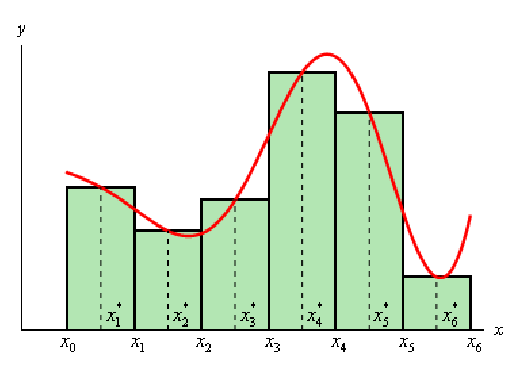
\includegraphics{lec19n-midpoint.eps}
 \caption{Schematic of midpoint rule.}
 \label{fig:midpoint}
 \end{marginfigure}
 
 Figure \ref{fig:midpoint} gives a simple illustration of the midpoint rule.  For the midpoint rule, the function $f(x)$ is approximated as a piece-wise constant.  Each piece of the piece-wise constant function is set to be equal to $f(x)$ at the midpoint of each sub-interval.\sidenote{These methods are only applicable for \emph{definite} integrals over $x\in(a,b)$. Also, unless otherwise noted, you should assume $a$ and $b$ are finite.}  It is not necessary that the sub-intervals be the same width but, in order to ease the implementation and to be consistent with common theoretical analysis, we will assume the sub-intervals are of equal length, which we will denote: $(x_i - x_{i-1})=h$.
 
 The integration formula is:
 \begin{align*}
 \int_{a}^{b} f(x) \ dx \approx \int_{a}^{b} g(x) \ dx &= \int_{x_0}^{x_1}f\left(\frac{x_1 + x_0}{2}\right) \ dx + \cdots + \int_{x_{n-1}}^{x_n}f\left(\frac{x_n + x_{n-1}}{2} \right) \ dx \\
 &= h \sum\limits_{i=1}^{n} f(m_i), \ \ m_i = \frac{x_i+x_{i-1}}{2} 
 \end{align*}
 
 A simple implementation of this formula into a MATLAB function is shown in the listing below.\marginnote{\textbf{Note:} This implementation doesn't allow the user to break the domain into unequal sub-intervals.  Think about how you could change the function---not just the body, but the inputs also---to allow non-uniform sub-interval sizes.  What benefits might such a feature bring?}
 \begin{lstlisting}[style=myMatlab,name=lec19n-midpoint]
 function y = midpoint(f,xMin,xMax,N)
% function y = midpoint(f,a,b,N)
% inputs:
% f -- function_handle.  Handle to the function to be integrated
% xMin -- scalar.  Lower bound of integration
% xMax -- scalar.  Upper bound of integration
% N -- scalar.  Number of subdivisions
% output:
% y -- scalar.  Approximate of the integral of f(x) from a to b.
xS = linspace(xMin,xMax,N+1);
xMid = (1/2)*(xS(1:(end-1))+xS(2:end));
h = xS(2)-xS(1);
y = h*sum(f(xMid));
end
 \end{lstlisting}
 
 \begin{marginfigure}
 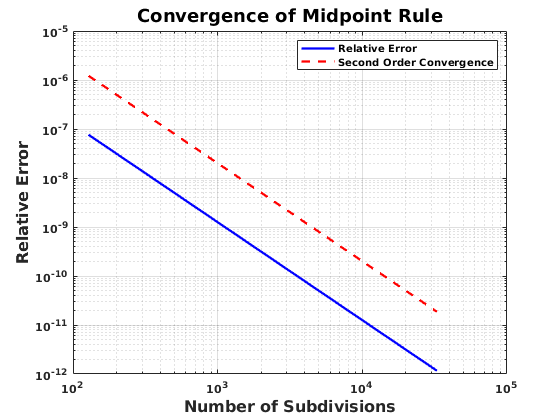
\includegraphics{lec19n-midpoint-convergence.png}
 \caption{Convergence of the midpoint rule.}
 \label{fig:lec19n-midpoint-convergence}
 \end{marginfigure}
 As is shown in Figure \ref{fig:lec19n-midpoint-convergence}, as the number of sub-intervals is increased, and thus $h$ decreases, the integration error is reduced.  For this method, the global error is $\mathcal{O}(h^2)$; meaning that the error can be bounded above by $C_0h^2$ where $C_0$ is a constant.  With this notation, by indicating the midpoint's global error is $\mathcal{O}(h^2)$ we say that the midpoint method is \emph{second order} convergent.
 
 \begin{marginfigure}
 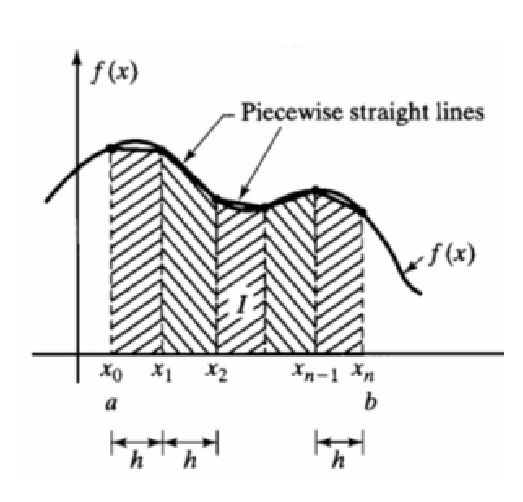
\includegraphics{lec19n-trapezoidal-rule.eps}
 \caption{Schematic of the trapezoidal rule with equal sub-interval sizes.}
 \label{fig:lec19n-trapezoidal-rule}
 \end{marginfigure}
 \subsection{Trapezoidal Rule}
 A schematic of the trapezoidal rule is shown in Figure \ref{fig:lec19n-trapezoidal-rule}.  The domain $[a,b]$ is broken into $n$ sub-intervals and the function $f(x)$ is approximated by a linear function within each sub-interval; the linear function $g(x)$ matches $f(x)$ at the end-points. As promised, integrating each of the simple functions within the domain is easy; each sub-interval is a trapezoid whose area can be calculated with a simple formula:
 %\begin{fullwidth}
 \begin{equation*}
 \int_{a}^{b} f(x) \ dx \approx \int_{a}^{b} g(x) \ dx = \int_{x_0}^{x_1} \frac{f(x_0)+f(x_1)}{2} \ dx + \cdots + \frac{f(x_{n-1})+ f(x_{n})}{2} \ dx
 \end{equation*} 
 %\end{fullwidth}
 
 As with the midpoint rule we will use equally-spaced sub-intervals: $x_{i}-x_{i-1}=h, \ i=1,2,\dots,n$ which results in the final form given in Equation \ref{eq:trapezoidal-rule}.
 \begin{equation}
 \int_{a}^{b} f(x) \ dx \approx h\left[\frac{f(x_0 = a)}{2} + \sum\limits_{i=1}^{n-1} f(x_i)+\frac{f(x_n = b)}{2} \right]
 \label{eq:trapezoidal-rule}
 \end{equation}
 Using this equation, we find that we can obtain second order convergence as shown in Figure \ref{fig:lec19n-trapezoidal-convergence}.
 \begin{marginfigure}
 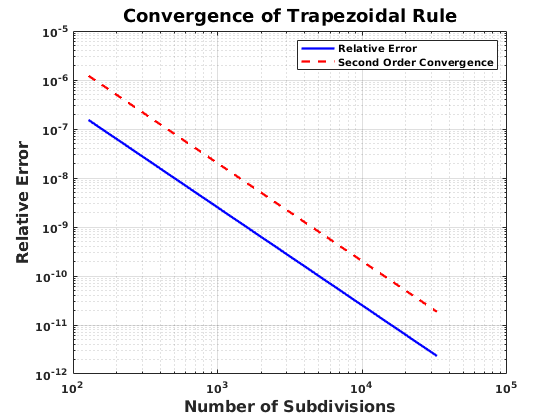
\includegraphics{lec19n-trapezoidal-convergence.png}
 \caption{Convergence behavior of the trapezoidal rule.}
 \label{fig:lec19n-trapezoidal-convergence}
 \end{marginfigure}


\subsection{Simpson's Rule}
\begin{marginfigure}
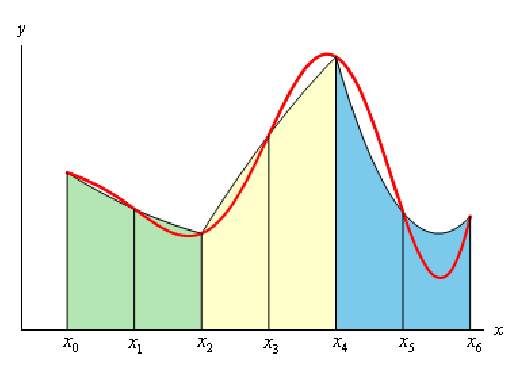
\includegraphics{lec19n-Simpsons-rule.eps}
\caption{Schematic of Simpson's rule.}
\label{fig:lec19n-Simpsons-rule}
\end{marginfigure}
In much the same way as with the midpoint and trapezoidal rules, Simpson's rule replaces $f(x)$ with a function that can be easily integrated; in this case a quadratic function.  The method is schematically shown in Figure \ref{fig:lec19n-Simpsons-rule}.  We partition the domain into an even number of sub-intervals (odd number of discrete points) each of equal length.  The function $g(x)$ is defined as:
\begin{equation*}
g(x) = c_0 + c_1x + c_2 x^2
\end{equation*}
We make $g(x)$ ``close'' to $f(x)$ by requiring $g(x_i) = f(x_i)$ at each partitioning point, $x_i$.  With some tedious algebra and calculus it can be shown that a unique function $g(x)$ meeting these conditions can be found and that its integral over a subdomain is:
\begin{equation*}
\int_{x_{i-1}}^{x_{i+1}} f(x) \ dx \approx \int_{x_{i-1}}^{x_{i+1}} g(x) \ dx = \frac{h}{3}\left[f(x_{i-1})+4f(x_i)+f(x_{i+1})\right] 
\end{equation*}
where $h = x_i - x_{i-1}$.
If we repeat this formula for all of the sub-intervals in $[a,b]$ we have the composite Simpson's rule formula as shown in Equation \ref{eq:lec19n-Simpsons-rule}.
\begin{equation}
\int_{a}^{b}f(x) \ dx \approx \frac{h}{3} \left[f(a) + 4 \sum\limits_{i=2,4,\dots}^{n-1} f(x_i) + 2 \sum\limits_{j=3,5,\dots}^{n} f(x_j) + f(b) \right]
\label{eq:lec19n-Simpsons-rule}
\end{equation}

An alternative derivation for Simpson's rule can be constructed by combining the midpoint and trapezoidal rules.  Careful inspection of Figure \ref{fig:lec19n-midpoint-convergence} and Figure \ref{fig:lec19n-trapezoidal-convergence} reveals that the midpoint rule is slightly more accurate than the trapezoidal rule. In fact, if you use both methods to integrate any quadratic polynomial using a single interval you will find that the error in the midpoint rule is \emph{exactly half} and \emph{opposite in sign} of the error when using the trapezoidal rule.\sidenote{Try it!!}  This suggests that one might get better accuracy if one combined the two methods: multiplying the midpoint rule result by $\sfrac{2}{3}$ and the trapezoidal rule result by $\sfrac{1}{3}$ and adding the results together, the error for any quadratic should go to zero!  If you follow this prescription:
\begin{align*}
\int_{a}^{b} f(x) &\approx \frac{2}{3} \text{midpoint rule} + \frac{1}{3} \text{trapezoidal rule} \\
&=\frac{2}{3} (2h)\left[f\left(\frac{a+b}{2}\right)\right]+\frac{1}{3}(2h)\left[\frac{f(a)+f(b)}{2}\right] \\
&=\frac{h}{3}\left[f(a) + 4f(\sfrac{a+b}{2})+f(b) \right]
\end{align*}
The last line of which is just Simpson's rule on a single interval.\sidenote{The factor $2h$ and $h$ appear because the original single interval for the midpoint and trapezoidal rules was formally subdivided to conform with the notation used in Simpson's rule.}

\begin{marginfigure}
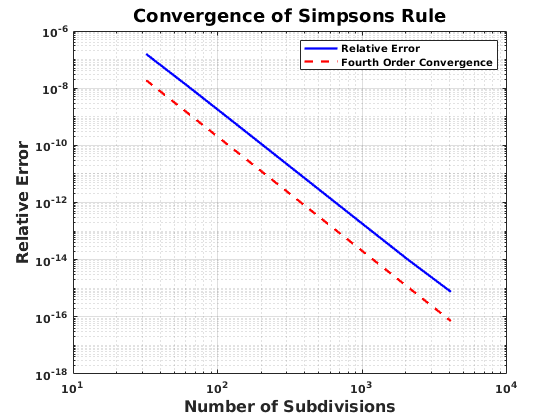
\includegraphics{lec19n-Simpsons-convergence.png}
\caption{Convergence behavior of Simpson's rule.}
\label{fig:lec19n-Simpsons-convergence}
\end{marginfigure}

The convergence behavior of Simpson's rule is shown in Figure \ref{fig:lec19n-Simpsons-convergence}. One thing that is not at all obvious from the previous discussion is: \emph{Why is Simpson's rule 4\textsuperscript{th}-order convergent?}  In particular, it is easy to verify that any \emph{cubic} polynomial will be integrated \emph{exactly} using Simpson's rule.  A logical way to see why this happens is to reformulate Simpson's rule as a \emph{numerical quadrature} rule.  Understanding this way of thinking will be useful for understanding the Gauss quadrature methods described in the next lecture.

\section{Numerical Quadrature}

In using numerical quadrature, we choose \emph{sample points} and \emph{weights} such that functions of increasingly higher order are integrated exactly.  We will show that Simpson's rule is equivalent to a numerical quadrature formula that allows us to integrate third-order polynomials exactly.\sidenote{Without loss of generality, we will assume that the interval of integration is $[0,1]$.  We can get back to the notation of Simpson's rule by multiplying the result by $2h$ since Simpson's rule must have, at a minimum, 2 sub-intervals which we will assume to be of equal length $h$.}  
\begin{align*}
\int_{0}^{1} f(x) \ dx &\approx \int_{a}^{b} g(x) \ dx = \sum\limits_{n=1}^{3} w_{i}g(x_i) \\
g(x) &= c_1 + c_1x + c_2x^2 + c_3x^3 
\end{align*}
Where $w_i$ are the weights, and $x_i$ are the sample points.  Our quadrature rule must satisfy:
\begin{align*}
\sum\limits_{i=1}^{3} w_{i}g(x_i) &= \overbrace{c_o\int_{0}^{1} 1 \ dx + c_1 \int_{0}^{1} x \ dx + c_2 \int_{0}^{1} x^2 \ dx + c_3 \int_{0}^{1} x^3 \ dx}^{\int_{0}^{1} g(x) \ dx} \\
\bracketMatrixstack{c_0 & c_1 & c_2 & c_3}\bracketMatrixstack{1 & 1 & 1 \\ x_1 & x_2 & x_3 \\ x_1^2 & x_2^2 & x_3^2 \\ x_1^3 & x_2^3 & x_3^3}\bracketVectorstack{w_1 \\ w_2 \\ w_3} &=\bracketMatrixstack{c_1 & c_1 & c_2 & c_3} \bracketVectorstack{\int_{0}^{1} 1 \ dx \\ \int_{0}^{1} x \ dx \\ \int_{0}^{1} x^2 \ dx \\ \int_{0}^{1} x^3 \ dx} = \bracketMatrixstack{c_1 & c_1 & c_2 & c_3}\bracketVectorstack{1 \\ \sfrac{1}{2} \\ \sfrac{1}{3} \\ \sfrac{1}{4}}
\end{align*}
Which results in the following nonlinear system of equations:
\begin{equation}
\bracketMatrixstack{1 & 1 & 1 \\ x_1 & x_2 & x_3 \\ x_1^2 & x_2^2 & x_3^2 \\ x_1^3 & x_2^3 & x_3^3}\bracketVectorstack{w_1 \\ w_2 \\ w_3} = \bracketVectorstack{1 \\ \sfrac{1}{2} \\ \sfrac{1}{3} \\ \sfrac{1}{4}}
\label{eq:lec19n-Simpson-Quad}
\end{equation}
In principle, the sample points and the weights are all unknown.  Let us simplify the problem and move a step closer to Simpson's rule by stipulating, at least, that $x_1 = 0$ and $x_3 = 1$.  This then leaves the middle sample point, $x_2$, and all of the are weights unknown.

We can analyze this using the MATLAB built-in function \lstinline[style=myMatlab]{fsolve}.

\begin{lstlisting}[style=myMatlab,name=lec19n-nq]
clear
clc
close all

% naive initial guesses
% xW(1) = x_2
% xW(2:4) = w_1, w_2, w_3
xW = [0.25 .25 0.25 0.25];

w = fsolve(quadRule,xW);

fprintf('The middle sample point is: x = %g.\n',w(1));
fprintf('The weights are: \n');
format long
disp(w(2:end))
format short




%% Local function for 
function w = quadRule(xW)

A = [1 1 1;
    0 xW(1) 1;
    0 xW(1)^2 1;
    0 xW(1)^3 1];

w = A*[xW(2);xW(3);xW(4)] - [1; 1/2; 1/3; 1/4];

end
\end{lstlisting}

\begin{marginfigure}
\includegraphics{lec19n-Simpsons-nleq.png}
\caption{MATLAB output to find middle sample point and all weights.}
\label{fig:lec19n-Simpsons-nleq}
\end{marginfigure}

Output from this script is shown in Figure \ref{fig:lec19n-Simpsons-nleq} indicating that, in order to exactly integrate a cubic polynomial, the sample point $x_2$ should be at the midpoint of the domain, and that the weights should be: $[\sfrac{1}{6}, \sfrac{2}{3}, \sfrac{1}{6}]$.  When we shift the interval to $[a,b]$ which is of length $2h$, we recover Simpson's rule.  This explains the observed convergence behavior.

Other quadrature formulas can be obtained using the exact same procedure.  For example, a 3-point quadrature formula that will exactly integrate 5th-order polynomials and (presumably) exhibit 6th-order convergence can be found by solving the non-linear equations:
\begin{equation}
\bracketMatrixstack{1 & 1 & 1 \\ x_1 & x_2 & x_3 \\ x_1^2 & x_2^2 & x_3 ^2 \\ x_1^3 & x_2^3 & x_3^3 \\ x_1^4 & x_2^4 & x_3^4 \\ x_1^5 & x_2^5 & x_3^5 }\bracketVectorstack{w_1 \\ w_2 \\ w_3} = \bracketVectorstack{1 \\ \sfrac{1}{2} \\ \sfrac{1}{3} \\ \sfrac{1}{4} \\ \sfrac{1}{5} \\ \sfrac{1}{6}}
\end{equation}
where all of the sample points and weights are unknown.  This system of equations can be solved to obtain the sample points and weights that are shown in Table \ref{tab:lec19n-3pt6th}. Convergence behavior is shown in Figure \ref{fig:lec19n-3p6o-convergence}.
\begin{margintable}
\begin{tabular}{|c|c|c|}
\hline
$i$ & $x_i$ & $w_i$ \\ \hline
1 & 0.1127016653792583 & 0.2777777777777786 \\ \hline
2 & 0.5 & 0.444444444444444493 \\ \hline
3 & $1-x_1$ & $w_1$ \\ \hline
\end{tabular}
\caption{Sample points and weights for a 3-point, 6th order convergent quadrature formula.}
\label{tab:lec19n-3pt6th}
\end{margintable}


\begin{marginfigure}
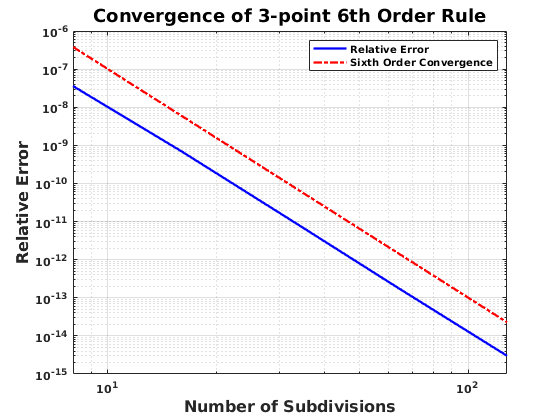
\includegraphics{lec19n-3p6o-convergence.png}
\caption{Convergence behavior of a 3-point, 6th order quadrature formula.}
\label{fig:lec19n-3p6o-convergence}
\end{marginfigure}
For three sample points and three weights, exact integration of 5th order polynomials and the associated 6th order convergence is the best you can do.  It turns out that the sample points and weights derived for this integrating rule are equivalent to those that will be derived in the next lecture, which is on Gauss quadrature, though the method used in the formulation is different.








